%----------------------------------------
% IT IS RECOMMENDED TO USE AUTOLATEX FOR
% COMPILING THIS DOCUMENT.
% http://www.arakhne.org/autolatex
%----------------------------------------

\documentclass[article,english,nodocumentinfo,nosayenslogo,noicartslogo]{utbmciadreport}

% The TeX code is entering with UTF8
% character encoding (Linux and MacOS standards)
\usepackage[utf8]{inputenc}
\usepackage{fancyhdr}
\usepackage{../common/sarl-colorized-listing}
\usepackage{graphicx}
\usepackage{url}

\graphicspath{{imgs/auto/},{imgs/},{../common/}}




\declaredocument{Introduction to MABS and Creation of a PacMan Game}{Lab Works MABS}{UTBM-INFO-AI51-LW-MABS}

\addauthorvalidator*[St\'ephane Galland]{St{\'e}phane}{Galland}{Teacher}

\updateversion{1.0}{\makedate{20}{01}{2016}}{First release on Github}{\upmpublic}
\incversion{\makedate{19}{03}{2020}}{Update the format}{\upmpublic}
\incversion{\makedate{26}{10}{2023}}{Update the sections}{\upmpublic}

\newif\ifCODESKELETON
\CODESKELETONtrue

\newif\ifJANUSINCLASSPATH
\JANUSINCLASSPATHfalse


\gdef\skeletonName{\texttt{\mbox{LW\_MABS\_skeleton\string.jar}}}



\begin{document}

\section{Goal of this Lab Work Session}

The goals of this lab work session are to:
\begin{itemize}
%\item introduce the basics concepts of agent-oriented programming with SARL, and
\item create a simple Pacman game.
\end{itemize}

You shall learn: 
\begin{itemize}
%\item regarding Goal 1:
%	\begin{itemize}
%	\item How to write the agent.
%	\item How to call an agent capacity.
%	\item How to spawn an agent from an agent.
%	\item How to define new capacities and skills.
%	\item How to exchange information between agents.
%	\end{itemize}
\item regarding Goal 1:
	\begin{itemize}
	\item What is the basics of a agent-based simulator.
	\item How to write the perception and action algorithms in the environment
	\item How to write the Ghost behavior.
	\end{itemize}
\end{itemize}

\section{First Step: prepare the development environment}

In this section, you will find the tasks to do for preparing your development environment.

\subsection{Installation of the Eclipse Tools}

\begin{emphbox}
Recommended version of SARL : \sarlversion
\end{emphbox}

\begin{enumerate}
\item Download the \Emph{Eclipse product} that contains the compilation tools for the SARL programming language : \url{http://www.sarl.io}
\item Uncompress the Eclipse product for SARL.
\item Launch the downloaded Eclipse product.
\item Open the wizard for creating a SARL project, with the menu: \\
	\texttt{> File > New > Project > SARL > Project}
\item Enter the name of the project.
%\item Click on the tab with the name \code{Libraries}.
%\item \textcolor{red}{In the list of the libraries, remove the \code{SARL Libraries}.}
%\item \textcolor{red}{In the list of the libraries, add the \code{Janus Libraries}} (the skeletons that are provided for this lab work has a dependency to an class that is provided by the Janus libraries).
\item Click on "Finish", the SARL project should be created.
%\item You must ensure that the configuration of your SARL project is correct:
%	\begin{enumerate}[a]
%	\item Open the dialog of the properties of the SARL project by clicking on: \\
%		\texttt{Right click on project > Properties > SARL > Compiler > Output Folder}
%	\item Check if the field ``Directory'' is set to a source folder that is existing in your SARL project. If not change the property with): \\
%		\texttt{src/main/generated-sources/sarl}
%	\end{enumerate}
\end{enumerate}

Your Eclipse is now ready for the lab work session. You should now install the code skeleton provided by the teachers.

\subsection{Installation of the Code Skeleton}

The teachers provide a code skeleton that should be completed by you for terminating the tasks related to this lab work session.
The steps to follow for installing the code skeleton are:
\begin{enumerate}
\item Download from the Teams of UTBM the file with the name \skeletonName.
\item Open the wizard for importing the code skeleton into the SARL project (right-click on the project name in the package explorer)	: \\
	\texttt{Right click on project > Import > General > Archive File}
\item Select on the local file system the downloaded file of the code skeleton; and click on ``Finish''.
\item The source folders of your project shall contains SARL and Java code. \\
	Some errors are appearing since they are related to the missed part of the code that must be provided by you. 
\item Clean the workspace for ensuring that every file is compiled: \\
	\texttt{Menu > Project > Clean}
\end{enumerate}

Figure \figref{eclipse_project_structure} on the page \figpageref{eclipse_project_structure} gives an example of the structure of the SARL project that you should obtain.

\mfigure[p]{width=.33\linewidth}{eclipse_project_structure}{Example of the structure of a SARL project}{eclipse_project_structure}



\section{Create a project}

For Linux and MacOS, there is nothing special to do.

For Windows operating system, I recommend to use the Maven (\url{http://maven.apache.org}) system in order to solve incompatiblities in URL computation within the Eclipse framework.

For creating a SARL project on Windows, you have to:
\begin{enumerate}
\item Open the dialog box, "File" $>$ "New" $>$ "Project";
\item Select the type of project: "Maven" $>$ "SARL Maven Project"; Click on "Next";
\item Check the box "Create a simple project"; Click on "Next";
\item Enter a group id and an artifact id; Click on "Finish";
\item Open the file "pom.xml" and edit it in order to add the following dependency:
\texttt{\string<dependencies\string>}\\
\texttt{\string<dependency\string>}\\
\texttt{\string<groupId\string>io.sarl.sre.janus\string</groupId\string>}\\
\texttt{\string<artifactId\string>janus.kernel\string</artifactId\string>}\\
\texttt{\string<version\string>3.0.13.0\string</version\string>}\\
\texttt{\string</dependency\string>}\\
\texttt{\string</dependencies\string>}
\item Right click on the project name $>$ "Maven" $>$ "Update project..."
\end{enumerate}

%\section{Introduction to the SARL Language}

%The following sections describe the work to be done during this lab work session regarding the introduction to the SARL language.

%SARL is a statically-typed agent-programming language.
%It aims at providing the fundamental abstractions for dealing with concurrency, distribution, interaction, decentralization, reactivity, autonomy and dynamic reconfiguration.
%These high-level features are now considered as the major requirements for an easy and practical implementation of modern complex software applications that are including intelligent behaviors.
%Authors of SARL are convinced that the agent-oriented paradigm holds the keys to effectively meet this challenge.

%Syntactically and semantically SARL has its roots in the Java programming language but improves on many aspects:
%\begin{description}
%\item[Agent specific statements] provide specific statements for agent programming (\href{http://www.sarl.io/docs/official/index.html\#5-2-agent-oriented-programming}{documentation});
%\item[Type inference] you rarely need to write down type signatures anymore (\href{http://www.sarl.io/docs/official/reference/GeneralSyntax.html}{documentation});
%\item[Lambda expressions] concise syntax for anonymous function literals (\href{http://www.sarl.io/docs/official/reference/general/Lambda.html}{documentation});
%\item[Operator overloading] make your libraries even more expressive (\href{http://www.sarl.io/docs/official/reference/general/Operators.html}{documentation});
%\item[Extension methods] enhance closed types with new functionality (\href{http://www.sarl.io/docs/official/reference/general/Extension.html}{documentation});
%\item[Powerful switch expressions] type based switching with implicit casts (\href{http://www.sarl.io/docs/official/reference/general/SwitchExpression.html}{documentation});
%\item[No statements] everything is an expression (\href{http://www.sarl.io/docs/official/reference/GeneralSyntax.html\#4-details-on-the-sarl-language-elements}{documentation});
%\item[Full support for Java generics] including all conformance and conversion rules;
%\item[Translates to Java not bytecode] understand what is going on and use your code for platforms such as Android or GWT.
%\end{description}

%Unlike several of the other JVM languages, SARL has zero interoperability issues with Java: everything you write interacts with Java exactly as expected.
%At the same time, SARL is much more concise, readable and expressive.

%Of course, you can call SARL methods from Java, too, in a completely transparent way.
%Furthermore, SARL provides a modern Eclipse-based IDE closely integrated with the Eclipse Java Development Tools (JDT), including features like call-hierarchies, rename refactoring, debugging and many more.

%Nevertheless, and even if SARL is closely related to Java, the SARL compiler is able to generate code for other target languages, e.g. Python.

%For a brief comparison between SARL, Java, Xtend and Scala languages, see the Section "\href{http://www.sarl.io/docs/official/reference/OOP.html\#1-comparison-between-sarl-and-other-languages}{Comparison between SARL, Java and Xtend}".


%\subsection{First Agent}

%First, you should write an agent that is able to display ``Hello World'' on the output console.

%You should:
%\begin{enumerate}[a)]
%\item create the agent type with the name \code{Agent1} (with the wizard, or by hand).
%\item create the event handler that is run when the \code{Initialize} event is received by the agent. This event is fired by the platform when the agent should initializee itself.
%\item write the output statement in the event handler.
%\end{enumerate}

%For running the agent, you should:
%\begin{enumerate}[a)]
%\item Open the dialog box of the ``Run Configurations''.
%\item On the left side, click on ``SARL Agent''.
%\item Click on the ``New launch configuration'' button.
%\item On the right side, select the project and the agent to launch.
%\item Click on ``Run''.
%\end{enumerate}

%\Emph{It is recommended to put a breakpoint in the event handler, and run the agent in debug mode.}

%When launching, if you have an error, such "Boot class not found", please create your project as a SARL Maven project.
%If the error is still present, then you could launch the SARL program as a standard Java application:
%\begin{enumerate}
%\item Open the dialog box of the ``Run Configurations''.
%\item On the left side, click on ``Java Application''.
%\item Click on the ``New launch configuration'' button.
%\item On the right side, select the project.
%\item In the field "Main class", enter: \texttt{io.janusproject.Boot}
%\item Open the tab "Arguments", and enter the following command line argument into the "Program arguments" field: \\
%	\texttt{-o --nologo the\_package\_of\_your\_agent.name\_of\_your\_agent} \\
%	where \texttt{the\_package\_of\_your\_agent.name\_of\_your\_agent} is the fully qualified name of your agent.
%\item Click on ``Run''.
%\end{enumerate}

%\subsection{Use the Logging Buildin Capacity}

%The goal of this exercise is to use a capacity that is provided by the run-time platform, aka. buildin capacity.

%You should:
%\begin{enumerate}[a)]
%\item update the agent code for using the ``Logging'' capacity.
%\item May anything else be changed in the code?
%\end{enumerate}

%\subsection{Spawning Another Agent}

%Most of the time, a system is composed by more than one agent. This exercise will enable you to launch another agent that is displaying ``Welcome'' on the output console also.

%You should:
%\begin{enumerate}[a)]
%\item create a second agent \code{Agent2}, with its \code{Initialize} event handler that is displaying the welcome message.
%\item Update the code of \code{Agent1} for using the \code{DefaultContextInteractions} buildin capacity. This capacity permits to do something with the context in which the agent is living, aka. the default context.
%\item Update the \code{Initialize} event handler of \code{Agent1} for spawning an agent of type \code{Agent2}.
%\item create a third agent \code{Agent3}, with its \code{Initialize} event handler that is displaying the welcome message.
%\item Update the \code{Initialize} event handler of \code{Agent1} for spawning an agent of type \code{Agent3}.
%\end{enumerate}

%\subsection{Say Hello to Every Ones}

%Agents are social entities. They are supposed to interact with other agents.
%This exercice enables the \code{Agent1} to say hello to the other agents.

%In SARL, the information exchanged between agents are carried out by events.
%The events are put inside an interaction space of a context.
%In this exercise, the default space of the default context will be used.
%It is automatically accessible when using the \code{DefaultContextInteractions} capacity.

%You should:
%\begin{enumerate}[a)]
%\item create the definition of the event \code{Hello}.
%\item update the code of \code{Agent1} for sending the event to every one after it has spawned the other agents.
%\item update the code of \code{Agent2} and \code{Agent3} for displaying the welcome message when they are receiving the hello event.
%\end{enumerate}

%\subsection{Say Hello to a Single Agent}

%Broadcasting events may not be the interaction mode between two agents.
%In this exercise, the \code{Hello} message will be sent only to \code{Agent3}.

%You should:
%\begin{enumerate}[a)]
%\item update the code of \code{Agent1} for emiting the event with a scope retricted to \code{Agent3}.
%\end{enumerate}

%\subsection{Say Localized Welcome}

%Agents may have different ways for doing a specific task.
%In this exercise, the agents will be enable to say "Hello" according to their own skills, i.e. their languages.

%The concepts of Capacity and Skill are suitable for this task.
%A capacity is the definition of functions (similar to an interface in object-oriented programming) that could be invoked by the agents. A capacity never defines the code of a function, only its prototype.
%A skill is a specific implementation of a capacity (similar to object implementing an interface in object-oriented programming). The skill must provide a code for each function of the implemented capacity.

%You should:
%\begin{enumerate}[a)]
%\item define the \code{SayHello} capacity.
%\item define the \code{SayHelloSkill} skill, that permits to say hello in English.
%\item define the \code{DireBonjourSkill} skill, that permits to say hello in French.
%\item update the code of the agents, that are defined previously, for using the \code{SayHello} capacity.
%\item update the code of the agents for calling the function provided by the \code{SayHello} capacity.
%\item update \code{Initialize} event handler of \code{Agent2} for defining its skill that is corresponding to the \code{SayHello} capacity. It should speak English.
%\item update \code{Initialize} event handler of \code{Agent3} for defining its skill that is corresponding to the \code{SayHello} capacity. It should speak French.
%\end{enumerate}

%\subsection{Contract Net Protocol (optional)}

%In this excercise, you must define a multiagent system that is running a Contract Net Protocol:
%\begin{enumerate}
%\item A customer wants to by a product.
%\item The customer sends a request to a broker for finder the best provider.
%\item The broker asks to a couple of provider they offers for the product.
%\item The broker selects the best offer.
%\item The broker notifies the selected provider about its acceptance with the ID of the customer.
%\item The broker notifies the not selected providers about their rejections.
%\item The broker notifies the customer with the ID of the provider.
%\end{enumerate}

%You should:
%\begin{enumerate}[a)]
%\item Define the capacity of the provider.
%\item Define the capacities of the broker.
%\item Write the provider code.
%\item Write the broker code.
%\item Write the customer code.
%\end{enumerate}



\section{PacMan simulator}

\subsection{Installation of the Code Skeleton}

The teachers provide a code skeleton that should be completed by you for terminating the tasks related to this lab work session.
The steps to follow for installing the code skeleton are:
\begin{enumerate}
\item Download from the Teams of UTBM the file with the name \skeletonName.
\item Upack the file with the name \skeletonName\ into a folder on your file system.
\item Open the wizard for importing the unpacked code skeleton into the SARL project (right-click on the project name in the package explorer)	: \\
	\texttt{Right click on project > Import > General > SARL > Existing SARL Maven Project}
\item Select on the local file system the unpacked folder of the code skeleton; and click on ``Finish''.
\item The source folders of your project shall contains SARL code. \\
	Some errors are appearing since they are related to the missed part of the code that must be provided by you. 
\item Clean the workspace for ensuring that every file is compiled: \\
	\texttt{Menu > Project > Clean}
\end{enumerate}

Figure \ref{fig:eclipse_project_structure} on the page \pageref{fig:eclipse_project_structure} gives an example of the structure of the SARL project that you should obtain.

\begin{figure}[p]
	\centering
	\includegraphics[width=.33\linewidth]{eclipse_project_structure}
	\caption{Example of the structure of a SARL project}
	\label{fig:eclipse_project_structure}
\end{figure}

\subsection{General Architecture of the Pacman Simulator}

The code skeleton provides the implementation of basic simulator architecture, based on:
\begin{itemize}
\item The Environment is supported by a specific agent in order to benefit of the event-based communication provided by the \sarl language.
\item The definition of the environment content is the \code{Maze} class, which is an internal attribute of the environment agent.
\item Figure \ref{fig:simulator:arch} shows a general overview on the architecture.
\end{itemize}

\begin{figure}
	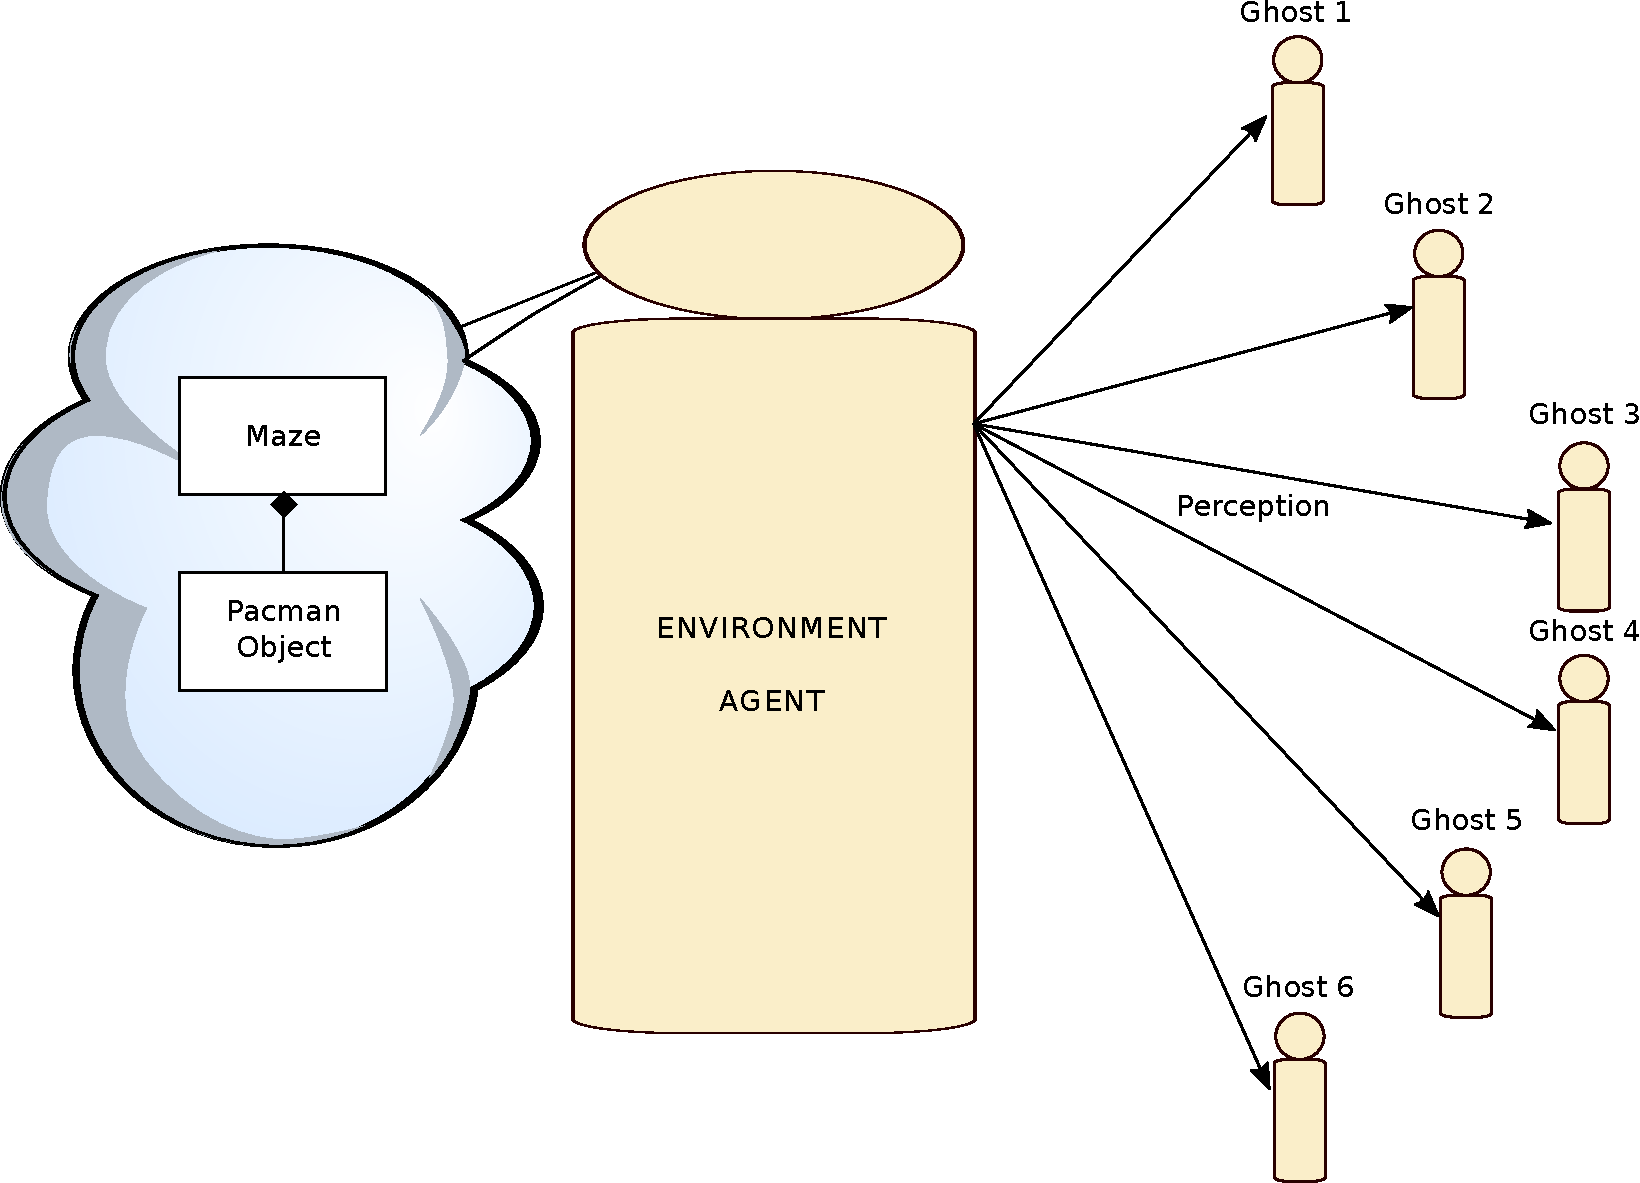
\includegraphics[width=.4\linewidth]{arch1}
	\hspace{1cm}
	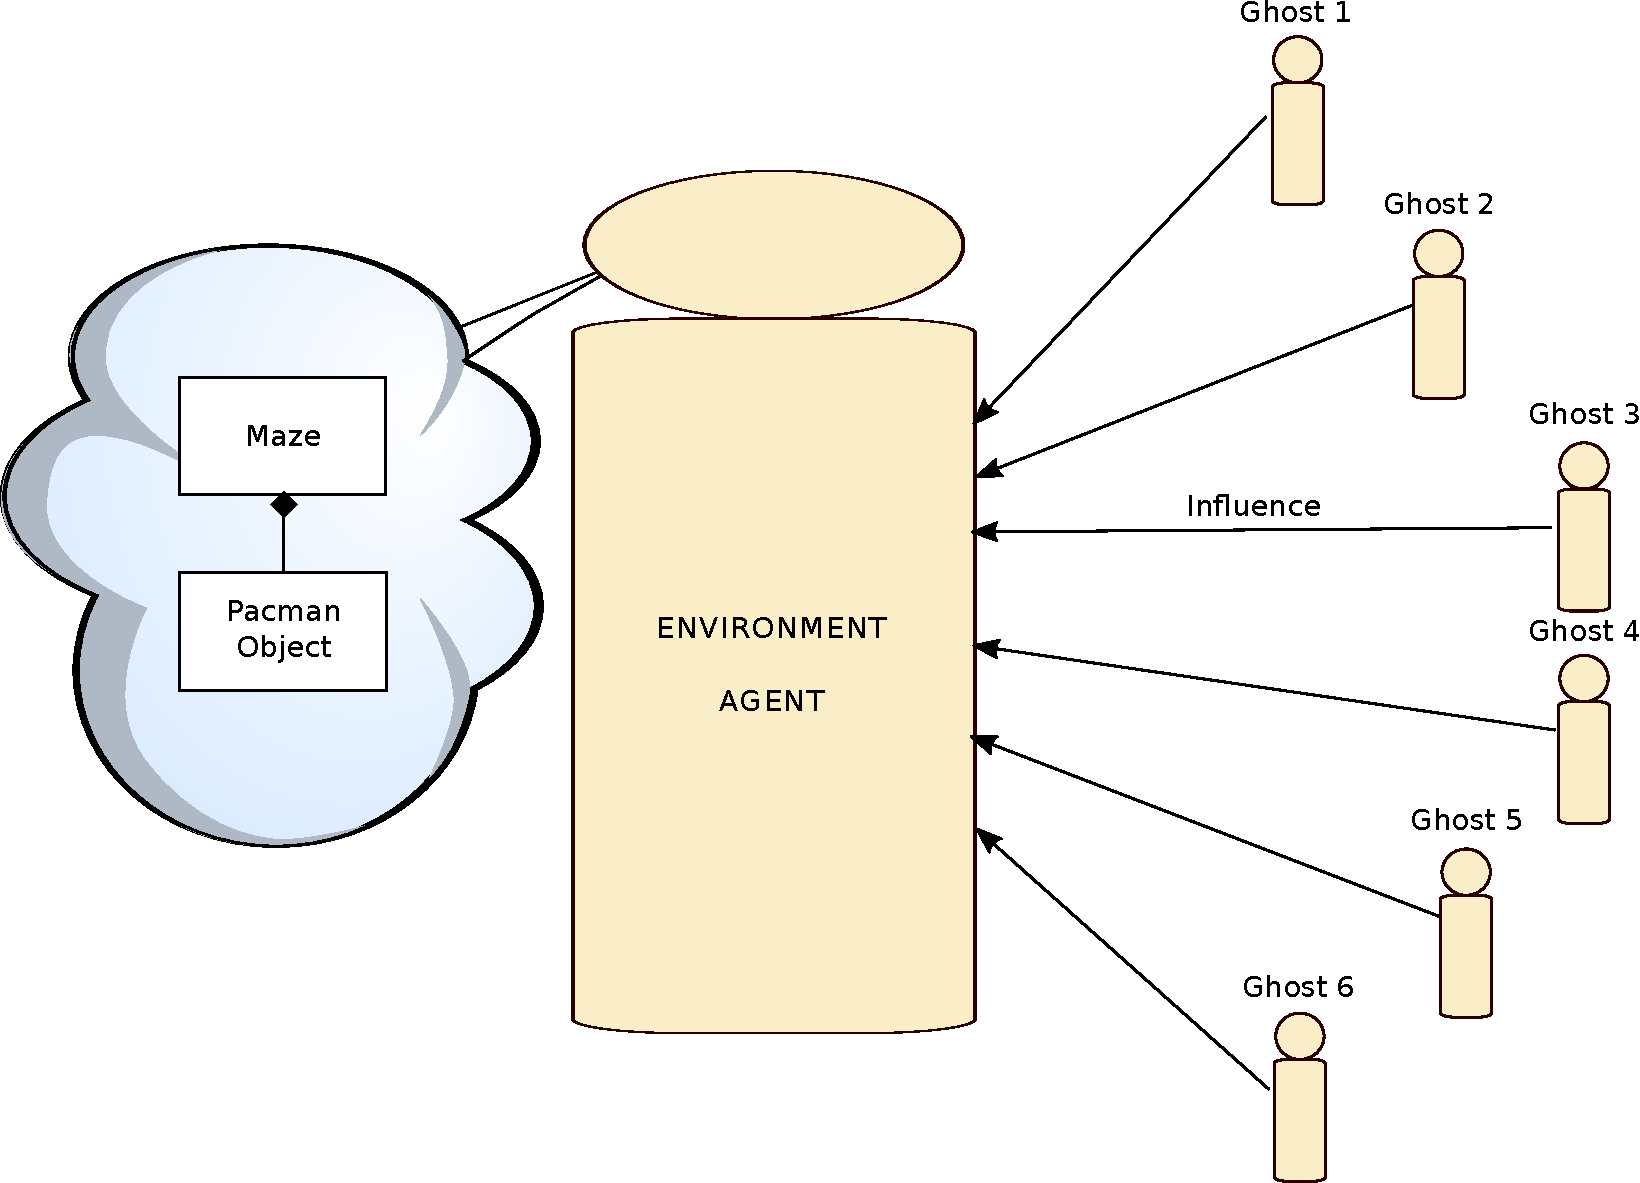
\includegraphics[width=.4\linewidth]{arch2}
	\caption{General Architecture of the Simulator. Left: sending perceptions to agents. Right: receiving influences from agents}
	\label{fig:simulator:arch}
\end{figure}

\subsection{Environment Perceptions}

In this excercise, you must define the algorithm for computing the perceptions.
\begin{enumerate}
\item Open the \texttt{fr/utbm/info/ia51/labworks/pacman/environment/agent/Environment.sarl} file.
\item Show the event handler \code{on RunBeginingOfStep}. This event is self-fired in order to start a step of the simulation loop. This function sends the perception events to the application agents.
\item Find the function which computes the perceptions, and open it.
\item Write the function code in the skill in order to compute the perceptions for each agent.
\end{enumerate}

\subsection{Environment Actions}

In this excercise, you must define the algorithm for applying the agents' actions into the environment.
\begin{enumerate}
\item Open the \texttt{fr/utbm/info/ia51/labworks/pacman/environment/agent/Environment.sarl} file.
\item Show the event handler \code{on RunEndOfStep}. This event is self-fired in order to finish a step of the simulation loop. This function tries to applied the influences sent by the application agents.
\item Find the function which tries to apply the influences, and open it.
\item Write the function code in the skill in order to detect conflicts, solve them, and change the state of the grid.
\end{enumerate}

\subsection{Ghost Behavior}

In this excercise, you must define the algorithm for the ghosts' behavior.
\begin{enumerate}
\item Open the \texttt{fr/utbm/info/ia51/labworks/pacman/players/Players.sarl} file.
\item Show the event handler \code{on Perception}. This event is received when the ghost agent should decide what to do.
\item Write the function code in the event handler in order to reproduce the following behavior:
	\begin{itemize}
	\item If the ghost perceives the Pacman body then
		\begin{itemize}
		\item If the pacman body has a super-power then flee
		\item Else pursue
		\end{itemize}
	\item Else
		\begin{itemize}
		\item If the ghost is at cross-road then select randomly a direction (the last selected direction should not be preferred).
		\item Else move forward.
		\end{itemize}
	\end{itemize}
\end{enumerate}

\end{document}
